\documentclass[10pt,twocolumn]{article}

\usepackage{pete}
\usepackage{times}
\usepackage{fullpage}
\usepackage{epsfig}
\usepackage{subfigure}
\usepackage{xspace}
\usepackage{amsmath}

\begin{document}

\title{\bf Scaling Strong Consistency Across Continents\\
with Hierarchical Consensus}
% \author{\rm{Benjamin Bengfort} and \rm{Pete Keleher}\\
% University of Maryland, College Park\\
% \{bengfort,keleher\}@cs.umd.edu}
\author{\emph{Omitted for review}}
\date{}

\maketitle

% Use the following at camera-ready time to suppress page numbers.
% Comment it out when you first submit the paper for review.
\thispagestyle{empty}

\begin{abstract}
    Eventually consistent systems can be made more consistent by reducing the time
until a write is fully replicated, improving global visibility of updates.
While gossip-based anti-entropy methods scale well, random selection of
anti-entropy partners is less than efficient.
Moreover, while eventual consistency may be consistent enough in a single data
center, geographic replication increases visibility latency and leads to
externally observable inconsistencies.
In this paper, we explore an improvement to pairwise, bilateral anti-entropy;
instead of uniform random selection, we introduce reinforcement learning
mechanisms to assign selection probabilities to replicas most likely to have
information.
The result is more efficient replication, faster visibility, and stronger
eventual consistency while maintaining high availability and partition
tolerance.

\end{abstract}

\section*{Introduction}

Coordination to ensure consistent behavior is essential to large-scale
distributed software systems, particularly modern systems that span
globe~\cite{spanner,mdcc,calvinfs,alvaro2013consistency}.
A range of mechanisms exist to provide varying levels of consistency, but
for systems that require strong guarantees, distributed consensus algorithms
are the primary technique for maintaining a correct global state across
independent machines in a computing cluster.
Consensus design traditionally considers primarily the requirement of
fault tolerance: progress in the face of one or two node failures.
Current approaches~\cite{mencius,epaxos,multicoordinated_paxos,spaxos}
therefore assume a small number of replicas in a co-located group, each
centrally located on a powerful and reliable host.
As a result, to scale modern systems that also have demanding requirements
for high throughput, low latency, and durability, consensus is typically used
in layers to manage smaller subsets of the system, trading performance for
reliability where possible.

% problem:
% - standard consensus doesn't scale well
% - it gets even worse across the wide area
% - current systems assume object-independence
% - current systems use fixed topographies and do not adapt

Systems that implement many small quorums of
coordination~\cite{mdcc,scatter,spanner} avoid the centralization bottleneck
and reliability concerns of master-service
systems~\cite{gray_dangers_1996,gfs} but create silos of independent
operation that are not coordinated with respect to each other.
Recently there has been increasing interest in dynamic and flexible quorums
to maintain decentralized ledgers~\cite{stellar} \fuzzy{but practical
experience shows that this results in the instantiation of a large number of
intersecting quorums}, which is not practical for a dedicated system that
does not have to worry about byzantine failure.

Most consensus algorithms have their roots in the Paxos~\cite{paxos}
algorithm, originally described in parliamentary terms.
The metaphor of government still applies well as we look at the evolution of
distributed coordination as systems have grown to include large numbers of
processes and geographies.
Systems that use a dedicated leader are easy to reason about and implement,
however, like chess, if the leader goes down the system cannot make any
progress.
Simple democracies for small groups solve this problem but do not scale, and
as the system grows, it fragments into tribes.
Inspired by modern governments, we propose a representative system of
consensus, such that replicas elect leaders to participate in a \roo that
makes decisions about the global state of the system.
Local decision making, the kind that effects only a subset of clients and
objects is handled locally by \subs as efficiently as possible.
The result is a a hierarchy of decision making that takes advantage of
hierarchies that already exist in applications.

% motivation:
% - hierarchies already exist in applications
% - geo-replication requires adaptivity
% - transactions don't work well with tablet structures
%   \pjk{We don't discuss them in this paper. Do we?}

In this paper, we describe \emph{Hierarchical Consensus (HC)}, an
implementation and extension of Vertical Paxos~\cite{vertical_paxos}.
Like Vertical Paxos, HC reasons about consistency across all objects by
identifying commands with a grid ordering (rather than a log ordering) and is
reconfigurable to adapt to dynamic environments that exist in geo-replicated
systems.
Adaptability allows HC to exploit locality of access, allowing for high
performance coordination, even with replication across the wide area.
HC extends Vertical Paxos to ensure that intersections exist between the
\subs and the \roo to ensure coordination exists between \subs and to ensure
that the system operates as a coordinated whole.
To scale the consensus protocol of the \roo, we propose a novel approach,
\emph{delegation}, to ensure that all replicas participate in consensus but
limit the number and frequency of messages required to achieve majority.
Finally, we generalize HC from primary-backup replication to describe more
general online replication required by distributed databases and file
systems.

% As always, the devil is in the details.
% In this paper we first walk through the consistency model, then discuss the
% components of the system in an understandable way by using Raft as our base
% consensus algorithm and a key/value store as our primary application.
% Most of the rest of a paper is a discussion of safety.
% How can things go wrong in such a system? What are the implications? How can
% the system adapt, remain resilient, and even outperform other fault tolerant
% distributed consensus?
% We conclude with an evaluation and a discussion of related works ...

The rest of the paper is organized as follows: we first describe the
background context that led to the intuition and motivations for HC,
primarily describing Raft~\cite{raft}, our consensus algorithm of choice and
a vertical consistency model.
We then describe the design of the system in detail and describe failure-free
operation of HC in a normal environment.
We follow the failure-free description with a description of how HC handles
various forms of failure and make an argument for the safety of the protocol,
including several specific cases of failure.
Finally we evaluate the performance of HC implemented as a distributed
key-value database, distributed across 15 geographic regions around the
world.

% claims:
% - HC is an implementation and extension of Vertical
%   Paxos~\cite{vertical_paxos} that organizes consensus hierarchically.
% - Use Raft~\cite{raft} for understandability
% - No requirement for SQ protocol to be Raft, however there must be \roo and
%   \sub intersections.
% - we assert that leader-oriented protocols work best.
% - generalized framework for scaling consensus

\section*{Background}



Paxos~\cite{fast_paxos,multicoordinated_paxos,generalized_paxos,epaxos,spaxos}
has two primary optimizations - fast path/slow path and leaders.

We implement and extend Vertical Paxos~\cite{vertical_paxos} but go beyond
primary backup replication to creating a key/value store (and soon a file
system).

Consider Niobe~\cite{niobe} and Boxwood~\cite{boxwood} as two implementations
of Vertical Paxos.

\subsection*{Raft Consensus}

A lightweight description of Raft and leader-oriented consensus protocols.

\subsection*{Vertical Consistency Model}

A command is identified by \texttt{(Epoch, Term, Log Index)} -- mirrors
Vertical Paxos \texttt{(Configuration, Ballot, Index)} structure.

Consistency: there must be a single, externalized ordering across all
objects.

Figure: grid ordering consistency.  \pjk{??}

\subsection*{Related Work}

\begin{itemize}
    \item ePaxos~\cite{epaxos} is best geo-replicated consensus, doesn't
    scale.
    \item MDCC~\cite{mdcc}, Spanner~\cite{spanner} are big systems across
    multiple data centers but isolate objects into tablets that aren't
    coordinated. \pjk{In what sense?  Does MDCC not re-configure tablets?}
    \item Niobe~\cite{niobe} and Boxwood~\cite{boxwood} are Vertical Paxos
    for primary replication but treat configuration as an independent master
    quorum and have independent object management.
\end{itemize}

\subsection*{HC Goals/Claims/Intuitions}

\strong{consistency claims:} We claim that for a current epoch, $E_i$,
this externalized ordering\footnote{\pjk{Hmm.. Externalized implies
    linearizability. Accesses will observe this, but that does not
    mean that we can rebuild it later on.  This comment seems to be
    more true for SC.}} exists
for all epochs $\leq E_{i-j}$ such that $j\geq1$ and $E_{i-j}$ is
\emph{closed}, e.g. a tombstone has been written to the logs of all \subs,
$S_{i-j}$.
In the current epoch, $E_i$ it is not possible to externalize a complete
ordering,  however it is possible to describe an observable sequential
ordering of all objects.

\strong{performance claims:} we should make some.

\begin{figure*}[hbtp]
  \centering
  \minipage{\textwidth}
      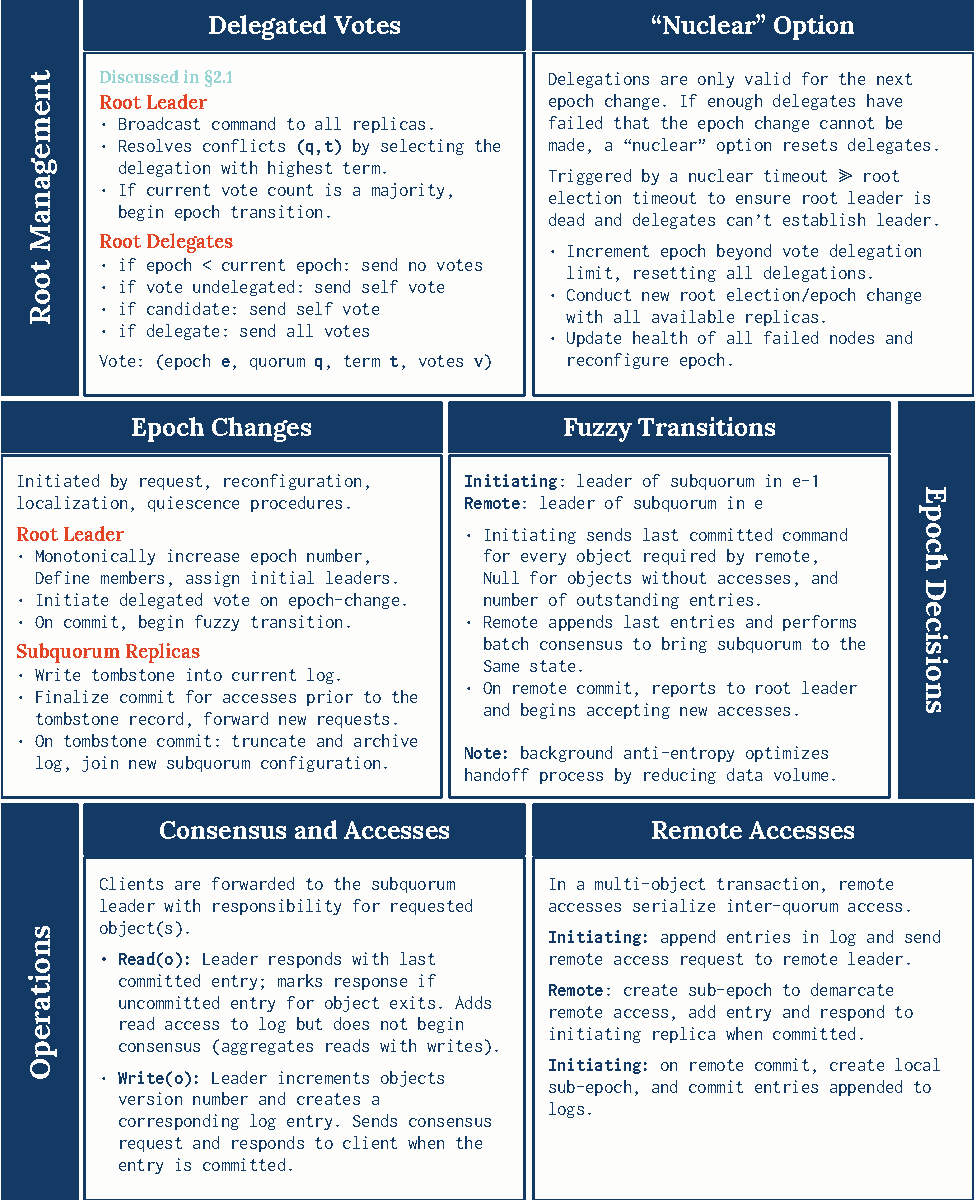
\includegraphics[width=\linewidth]{figures/hc_operation_summary}
      \caption{A condensed summary of the hierarchical consensus protocol. Operations are described in a top-to-bottom fashion where the top level is \roo operations, the bottom is \sub operations, and the middle is transition and intersection. Section numbers such as §5.2 indicate where particular features are discussed.}
      \label{fig:hc_operation_summary}
  \endminipage
\end{figure*}

\section*{Design}\footnote{\pjk{I'd make this a straw-man design, along the
  lines of SUNDR. We can then add delegation and generalized
  delegation later.}}

Preliminaries: a system is composed of a set of replicas, $R$, initially we
assume that this set is fixed, later we discuss adding or removing to this
set.
The system self organizes into a \roo.
The \roo assigns replicas to zero or one \subs.

During operation, a Replica can be \emph{one} of the following.

\begin{enumerate}
    \item A follower in a \sub
    \item A leader of a \sub and a member of the \roo
    \item A hot spare
\end{enumerate}

Replicas that are leaders can simultaneously be a \sub leader and a \roo
leader.
Later we relax this so that any replica can be a member of of the \roo.

\begin{figure}
    \centering
    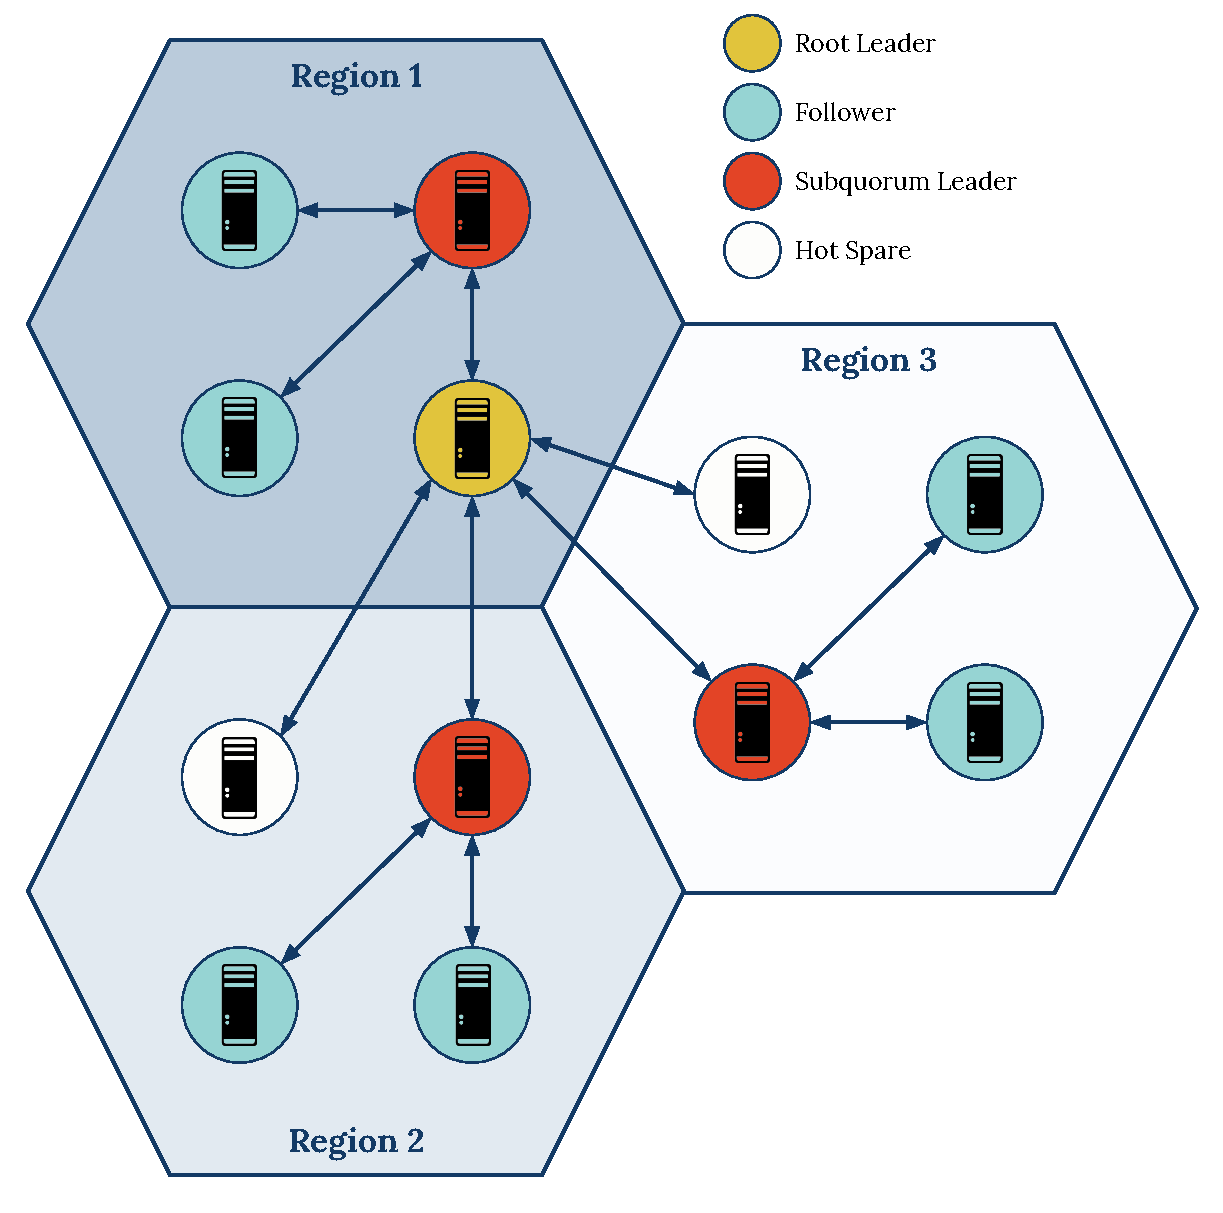
\includegraphics[width=0.5\textwidth]{figures/simple_example_topology}
    \caption{Simple Example: 12x3 HC Topology}
    \label{fig:simple_example_topology}
\end{figure}

\begin{figure*}
    \centering
    \minipage{\textwidth}
    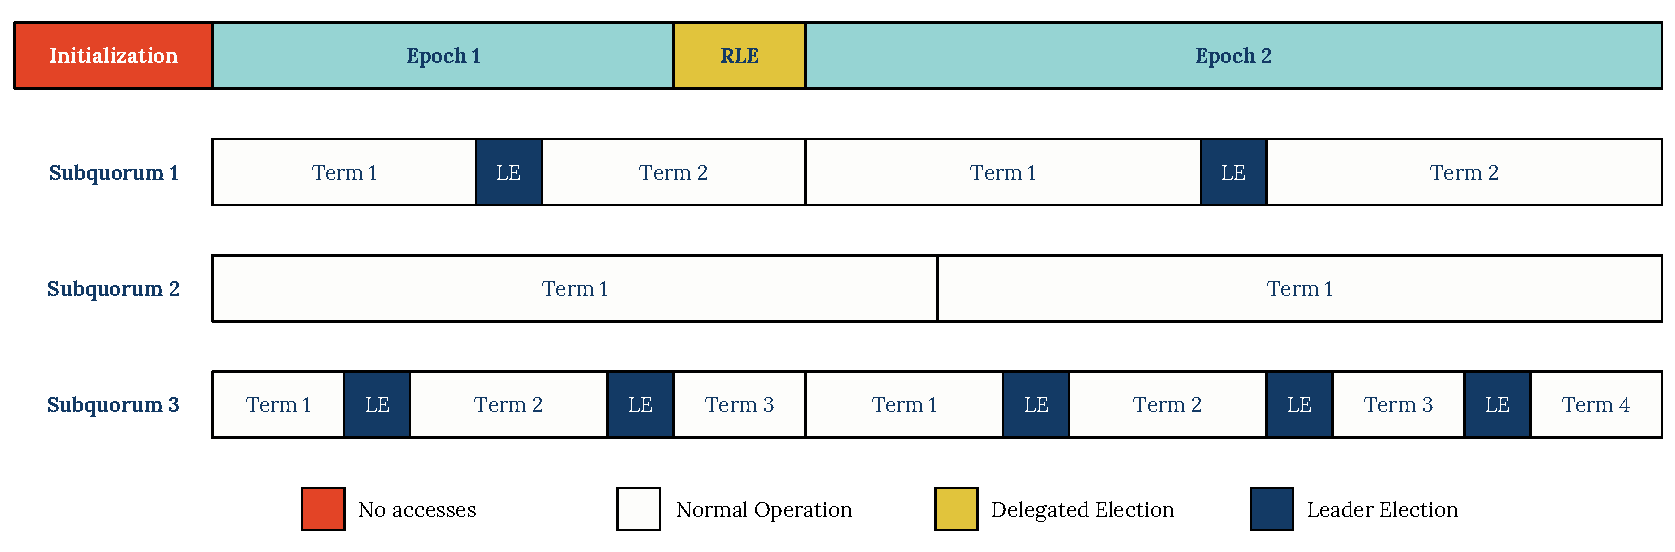
\includegraphics[width=\linewidth]{figures/simple_example_epochs_terms}
    \caption{Simple Example: Epochs and Terms Timeline}
    \label{fig:simple_example_epochs_terms}
    \endminipage
\end{figure*}

Another simple example

\begin{figure*}
    \centering
    \minipage{\textwidth}
    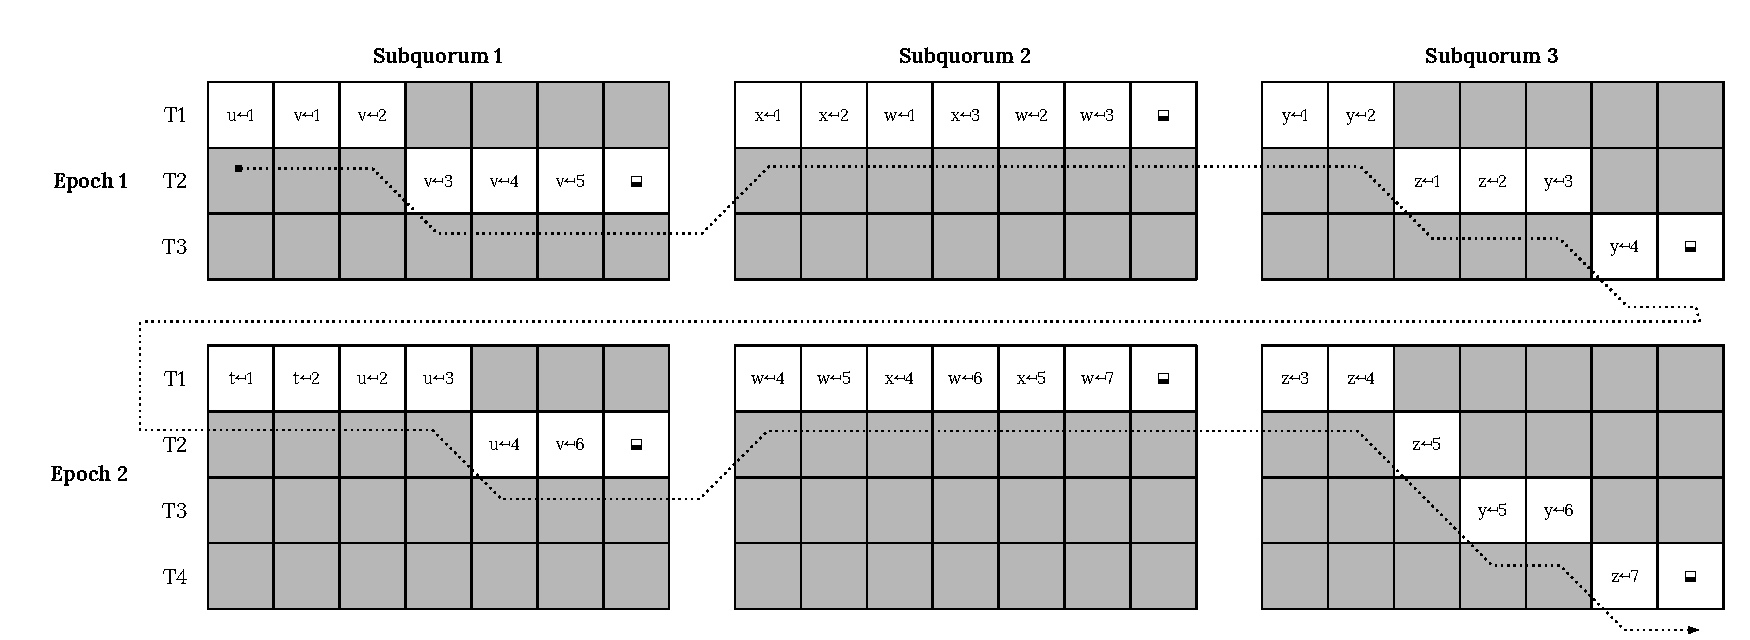
\includegraphics[width=\linewidth]{figures/simple_example_log_ordering}
    \caption{Simple Example: Log Ordering}
    \label{fig:simple_example_log_ordering}
    \endminipage
\end{figure*}

\subsection*{Elections and Delegation}

\begin{itemize}
    \item election of \roo leader
    \item assignment/election of \sub leaders
    \item delegation of votes
    \item re-elections
    \item delegations expire
\end{itemize}

\subsection*{Data Model}

\ben{maybe move this to a different location?}

\begin{itemize}
    \item key/value store
    \item read then write updates \pjk{We assume all writes
        implemented w/ read then write, or do we implement writes this
        way? And to what purpose?}
    \item accesses: get, put, delete
\end{itemize}

\subsection*{Operation/Decision Making}

\begin{itemize}
    \item \sub decision making
    \item remote reads and writes
    \item reconfiguration/epoch changes
    \item \roo decision making
    \item transitions/fuzzy epochs
\end{itemize}

\section*{Safety and Fault Tolerance}

\begin{itemize}
    \item individual faults
    \item partitions of the network (big faults)
    \item safety argument
\end{itemize}

\subsection*{Delegation Safety}

We have implemented two mechanisms for delegation safety: the first is
timeout based, and the second is a simple book-keeping mechanism.

In the timeout-based delegation, a replica delegates it's vote for a term
limited logical period, usually at least two epochs. This means that the
delegated vote lasts through at most 1 root leader election. The nuclear
timeout option is longer than the root election timeout, therefore in order
for the nuclear option to occur at least one failed root leader election also
must have occurred. Because the nuclear option is triggered after a root
leader election the delegation is reset on the nuclear option, and every
replica must vote for themselves (ensuring that the nuclear option contains
no delegations at all).

\pjk{Again, I think this fails if delegation can be used for root votes} In
the book-keeping mechanism, replicas can delegate their votes to anyone. All
root votes must be accompanied by the term, epoch, and ID of the delegation.
The root leader tracks votes as follows:

\begin{itemize}
\item If the delegated vote is not in the current epoch, it is discarded
\item Otherwise the leader accepts only the vote with the highest term (e.g.
the current subquorum leader).
\item If the leader receives a vote from the replica, then it accepts that
vote no matter what.
\end{itemize}

In this way, it is possible for duplicate votes to be received by the leader, but only a single vote per replica will be counted.

\subsection*{Assassination}

Scenario:

System size of 18, HC 5x3 (5 subquourms of size three, 3 hot spares) in 3 regions - 6 replicas per region. In epoch e there is a configuration such that all 5 subquorum leaders and the root leader are in a single region, which loses it's connectivity to the rest of the world. All followers have delegated their votes to their subquorum leaders, except the hot spares which haven't delegated to anyone.

Just a note here, we've been calling it "assassination" but it's actually very difficult to create a scenario where this occurs if replicas are evenly distributed over all regions without violating the principle of localization. In the above example, every single subquourm is geo-replicated.

6 replicas with 16 votes can communicate and 12 replicas with 2 votes cannot.

Step one: all subquorums elect a leader for the next term; they continue to handle requests.

Step two: group of 6 attempts an epoch change to repair the poor progress, they assign all work to two subquorums of 3 (best scenario if there is total failure).

Step three: group of 12 attempts a root leader election, it fails because they only have 2 votes.

Step four: group of 12 initiates nuclear option, taking back delegations, moves into an epoch after the group of 6.

We now have the scenario where we have concurrent writes to objects in two partitioned regions, however because of the epoch ordering, we know that all writes that happen in the group of 6 happen before the writes that happen in the group of 12.

The group of 6 cannot make another epoch change because their delegations have expired and they cannot re-acquire them.

\section*{Implementation and Evaluation}

\begin{itemize}
    \item Go implementation
    \item AWS EC2 across 15 regions and 150 replicas (3, size 3 subquorums in 15 regions with 15 hot spares).
    \item LevelDB
    \item Version numbers
\end{itemize}

Evaluation

\section*{Conclusion}

\begin{itemize}
    \item \todo{Psuedo code to make paper clearer}
    \item \bobby{Provide top down description, where each model is relatively small, reduce cognitive load}
    \item \bobby{Change name ``nuclear option'' -- make more technical e.g. ``final recovery'' (too jocular)}
\end{itemize}

\bibliography{bib}
\bibliographystyle{abbrv}

\end{document}
